%!TEX root = ../main.tex
\section{Modelling a DC motor}
This section deals with the modelling and parameterisation of a brushed DC motor, specifically the Pittmann 9234 24V servomotor.
Figure \ref{fig:dcmotormodel} is a simple model of a DC motor.
The parameters of this model will be estimated by experimentation.

\begin{figure}[!h]
	\centering
	\includegraphics[width=\linewidth]{graphics/dcmotormodel.png}
	\caption{Simulink model of a brushed DC motor.}
	\label{fig:dcmotormodel}
\end{figure}


\subsection{Armature Resistance - $R_a$}
The armature resistance, $R_a$ in figure \ref{fig:dcmotormodel}, can be found simply by applying Ohm's law.
The current through a resistor is well defined when a voltage is applied across it.
However, when the rotor is spinning, the circuit produces back-EMF.
This counters the input voltage, effectively lowering the current through $R_a$.
In order to avoid this effect the rotor is blocked.
Since, with a blocked rotor, there will be no change in voltage in the system, the inductor acts as a short circuit, reducing the circuit to a voltage across a resistor. 

\begin{figure}[!h]
	\centering
	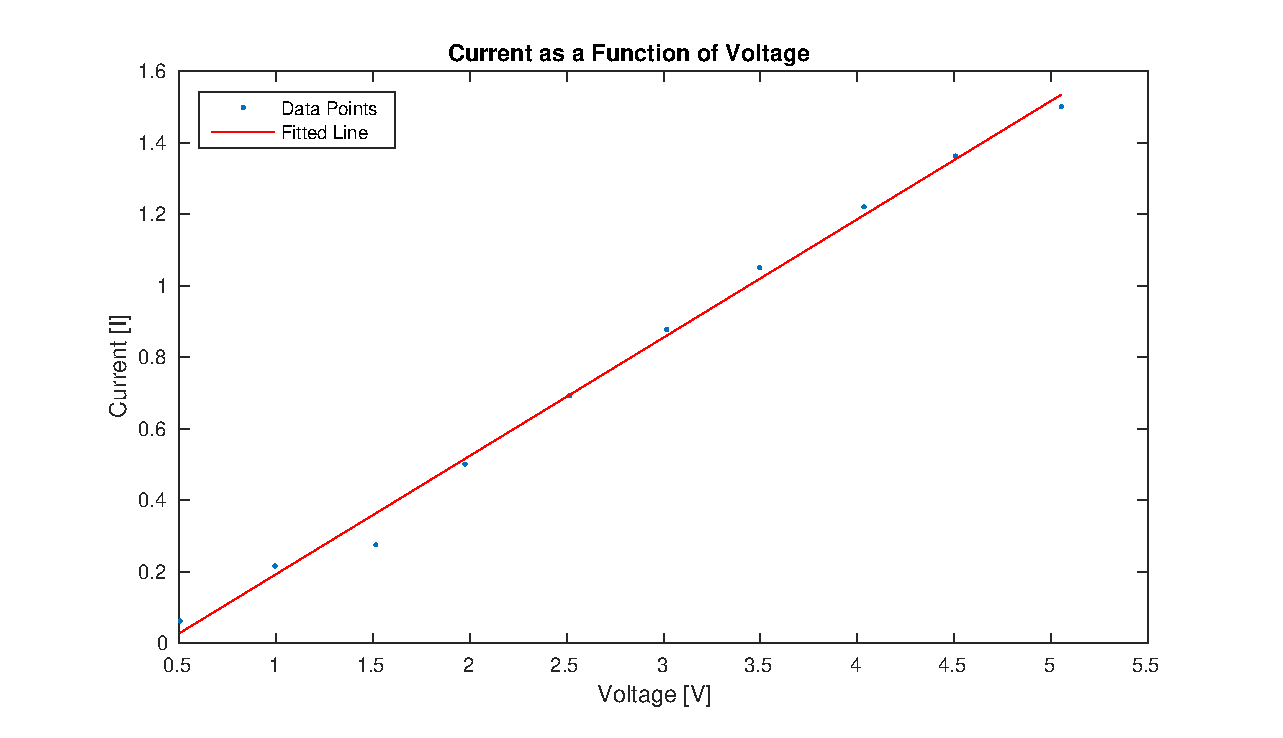
\includegraphics[width=\linewidth]{graphics/raplot}
	\caption{Current as a function of voltage with the rotor blocked.}
	\label{fig:raplot}
\end{figure}